%% master tex file for Needs Assessment Report

\documentclass{needs}

% header
% sample Policy header file

\orgname{Some Good Organization} % 
\reldate{May 5, 2017} % NEW

% Overview
\chartfile{./graphics/chart.png} % filename with path
\totRiskLevel{Medium} % Low, Medium, High
\totRiskScore{61} % []0-100%]

% Information Security Fundamentals table
\fOne{Deficient} % Deficient, Passing
\fTwo{Deficient}
\fThree{Passing}
\fFour{Passing}
\fFive{Deficient}
\fSix{Deficient}
\fSeven{Passing}
\fEight{Deficient}
\fNine{Passing}
\fTen{Passing}
\fEleven{Passing}
\fTwelve{Passing}
\fThirteen{Passing}
\fFourteen{Deficient}
\fFifteen{Passing}

% Focus Area 01 table
\areaOneRiskLevel{Medium} % Low, Medium, High
\areaOneScore{65} % [%] 0-100
\areaOneRec{Consider formalizing your risk assessment framework.} % pipe-separated list

% Focus Area 02 table
\areaTwoRiskLevel{High}
\areaTwoScore{33}
\areaTwoRec{Adopt a formal Information Security Policy |
	Adopt a formal Acceptable Use Policy
	}%

% Focus Area 03 table
\areaThreeRiskLevel{High}
\areaThreeScore{47}
\areaThreeRec{Formalize  your individual pieces of a program into a formal Information Security Program |
	Consider implementing a formal update schedule for your organizational policies |
	Consider having an outside third party review your organization's Information Security posture on a periodic basis |
	The methods that vendors and third parties use to protect your data are as important as the method and controls you use.  Assess your vendors' Information Security programs before conducting business |
	Consider making the protection of your organization's information a part of your vendor contracts
	}%

% Focus Area 04 table
\areaFourRiskLevel{High}
\areaFourScore{5}
\areaFourRec{Consider formalizing your Data Classification Guidelines |
	Organizational assets and information should be clearly labeled and identified according to your Data Classification Guidelines
	} %

% Focus Area 05 table
\areaFiveRiskLevel{tbd}
\areaFiveScore{0}
\areaFiveRec{tbd}

% Focus Area 06 table
\areaSixRiskLevel{tbd}
\areaSixScore{0}
\areaSixRec{tbd}

% Focus Area 07 table
\areaSevenRiskLevel{Medium}
\areaSevenScore{74}
\areaSevenRec{Careless disposal of information is a leading cause of data breaches.  Make sure that all media and information is securely destroyed before disposal or reuse |
	Consider setting your antivirus solution to update and run at least once per week on your workstations. |
	Consider implementing formal change control procedures to evaluate and if necessary roll back changes made to the organization's systems. |
	Consider archiving audit logs for all user activity as appropriate.  Audit logs make both troubleshooting and investigations easier and less time consuming. |
	Assign someone to review your audit logs on a periodic basis.  Many instances of fraud have been uncovered by a casual glance at log files. |
	Test your backup media from time to time, especially if you are using cassette media.  Backup media has a finite lifespan and must be replaced periodically. |
	Consider whether you really need sensitive personal information to be stored on laptop computers.  In cases where the answer is yes, continue with whole disk encryption. |
	Consider whether or not business applications really require sensitive personal information to be collected via the web.  In cases where the answer is yes, ensure that you continue the use of appropriate encryption. |
	Consider formally testing your websites for common vulnerabilities on a periodic basis. |
	Consider whether or not your business really needs to store credit card information.  In cases where the answer is yes, continue the use of appropriate encryption.
	} %

% Focus Area 08 table
\areaEightRiskLevel{tbd}
\areaEightScore{0}
\areaEightRec{tbd}

% Focus Area 09 table
\areaNineRiskLevel{tbd}
\areaNineScore{0}
\areaNineRec{tbd}

% Focus Area 10 table
\areaTenRiskLevel{tbd}
\areaTenScore{0}
\areaTenRec{tbd}

% Focus Area 11 table
\areaElevenRiskLevel{tbd}
\areaElevenScore{0}
\areaElevenRec{tbd}

% Focus Area 12 table
\areaTwelveRiskLevel{tbd}
\areaTwelveScore{0}
\areaTwelveRec{tbd}

% Next Steps list
\nextSteps{Stop to smell the roses. |
	Call your mother. |
	Do the next thing on your bucket list.
	}
 % custom inputs file

\begin{document}
		\maketitle
		
		\tableofcontents

	% page 1
%	\titleline
	
%	\doctable
	
%	\vfill
	\section{Introduction}
		Thank you for taking the time to complete this Needs Assessment Survey.  We look forward to helping you understand your own unique strengths and needs. Over the next few pages we will examine your answers in relation to how they contribute to your overall threat profile.  This report will help you understand what risks your business face, and make suggestions for improving your Information Security Program.
		
		Many organizations report feeling a bit overwhelmed after reading this report.  This is normal when you are starting to build your Information Security Program.  Rest assured that you are not alone in this feeling, and that it is easy to overcome it once you get started in addressing your particular needs – especially when you have someone to guide you through the process.
		
		It should be noted that this Needs Assessment should not be substituted for a full risk assessment.  For this assessment, we are relying solely on information you have provided us, and have not done anything further to verify this data.  
		
		Finally, we welcome the opportunity to discuss this report with you.  We know that sometimes starting down the path to securing your information seems fraught with obstacles.  We have helped thousands of clients secure their information.  And, we will be happy to help you get started in securing yours.
	
	\section{Overview of Results}
	
		\begin{figure}[h]
			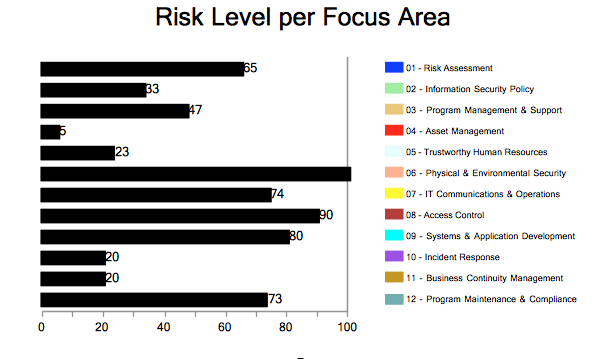
\includegraphics[width = 1\textwidth]{chart.png}
	%		\caption{chart}
		\end{figure}
		
		\overallResults
	
	\section{Information Security Fundamentals}
		Information Security can seem very complex.  For most organizations however, there are some fundamental items that when implemented correctly will cover most of your Information Security needs.  Every organization, regardless of size or complexity needs to have these items in place.  Because of this necessity, \theauthor uses this as a starting place for assessment.  As a practical take away, if you find yourself deficient in these fundamentals, you need to start here before focusing elsewhere.
	
	\infoTable
	
	\section{Detailed Risk Analysis}
		
		The following sections will analyze your strengths and needs in each of the focus areas of Information Security.  Each focus area is important and contributes to the overall effectiveness of your Information Security program.  Focusing too much on one area while neglecting another area can leave your organization vulnerable to information crimes.
		
		It should be noted that this Needs Assessment is meant to give the user a quick snapshot of their Information Security Program, and is not intended to replace a full enterprise risk assessment by a certified auditor.  
	
	\section{Focus Area 01 -- Risk Assessment}
	
		Risk assessment is the foundation of information security planning.  If your organization’s Information Security Program is going to be effective, the program must address the unique risks faced by your organization.  Risks must be fully identified and understood before effective mitigation strategies can be developed.  Risk assessment addresses both the process of identifying vulnerabilities and threats as well as the probabilities of their occurrence and potential impact.
		
		Your Information Security Program should include at least the following: 
		\begin{checklist}
			\item A framework for the identification and quantification of risks to your organization
			\item A strategy for developing mitigation strategies to address risks to your organization
			\item Periodic review and update of your risk assessment
		\end{checklist}	
		
		\vspace{20pt}
		\fOneTable
		
	\section{Focus Area 02 -- Information Security Policy}
	
		Documentation of policy is imperative in outlining the principles of any Information Security Program.  These policies address management directives for establishing information security for the organization, identify relevant contracts, laws and regulations constraining the organization, and sets procedures to be used in day-to-day operations.
		
		An effective set of Information Security policies should include at least the following: 
		\begin{checklist}
			\item Establishment of an Information Security Policy
			\item Establishment of an Employee Handbook
			\item Establishment of a Review Schedule for appropriate policies
		\end{checklist}
		
		\vspace{20pt}
		\fTwoTable
				
	\section{Focus Area 03 -- Program Management and Support}
	
		All information security responsibilities should be defined for employees and addressed appropriately with external parties.  An effective Information Security Program requires a supporting structure within the organization as well as necessary controls for customers, contractors, or partners to sustain a successful information security program.
		
		Your Information Security Program should include at least the following: 
		\begin{checklist}
			\item To organize the support structures for an effective information security program
			\item Ensuring management’s support for information security
			\item Coordination of information security roles and the allocation of responsibilities among staff
			\item Establishment of authorization processes
			\item Establishment of Non-Disclosure policies and confidentiality agreements
			\item Establishment of relationships with external parties and special interest groups
			\item Management of external relationships
		\end{checklist}		
	
		\vspace{20pt}
		\fThreeTable
		
	\section{Focus Area 04 - Asset Management}
	
		Just like risk assessment, you can’t protect something if you don’t know you have it. As an essential part of risk management and disaster recovery, an inventory of assets and information should be maintained by the organization.  Without it, the organization has no idea what it is protecting. An effective program should contain guidelines for data owners, classification guidelines, labeling and handling guidelines and establish the acceptable use of information.
		
		Your Information Security Program should include at least the following: 
		\begin{checklist}
			\item Establish an asset inventory
			\item Implementation of classification guidelines
			\item Identifying owners for the organization’s information and assets
			\item Establishing Information Labeling and Handling Policies
			\item Establishing an Acceptable Use Policy
		\end{checklist}	
		
		\vspace{20pt}
		\fFourTable
		
	\section{Focus Area 05 - Trustworthy Human Resources}
	
		Protection of information cannot be expected by default. Employees, contractors, vendors and other related third parties each have obligations to protect your organization’s information.  Beginning with trustworthy personnel, the organization should offer training for defined information security expectations and have a disciplinary plan for handling information security incidents.
		
		Your Information Security Program should include at least the following human resource concerns: 
		\begin{checklist}
			\item Documentation of roles and responsibilities
			\item Establishment of a background screening policy
			\item Review of Terms and Conditions of employment
			\item Implementation of Information Security Awareness, Education and Training
			\item Establishment of formal disciplinary and termination processes
		\end{checklist}
		
		\vspace{20pt}
		\fFiveTable	
		
	\section{Focus Area 06 - Physical and Environmental Security}
	
		Proper concern should be given to physical and environmental threats that are either natural or man-made.  Everything from the physical perimeter, placement of equipment storing sensitive information and contingency plans for environmental disasters must be assessed.  This section highlights characteristics to consider for protecting the organization’s information security from such issues.
		
		Your Information Security Program should include at least the following: 
		\begin{checklist}
			\item Assessment of the physical security perimeter
			\item Evaluation of physical entry controls, office security, external and environmental threats, public areas and loading docks, supporting utilities and cabling
			\item Assessment of equipment security located offsite
			\item Establishment of Information Disposal and Reuse policies
			\item Controlling the removal of property
		\end{checklist}
		
		\vspace{20pt}
		\fSixTable
		
	\section{Focus Area 07 – Information Technology Communications and Operations}
		
		Today’s business environment relies on networked computer systems to retain, process, and produce immense amounts of information.   Attention needs to be given to ensuring that these assets protect your organization’s information as opposed to creating a liability.  Appropriately secure systems need to be properly configured, have documented operating procedures and audit trails.  
		
		Your Information Security Program should include at least the following: 
		\begin{itemize}
			\item Evaluation of operating procedures
			\item Establishment of operating policies including change control, segregation of duties, separation of production systems, capacity management, system acceptance, malicious code, mobile code, information backup and media disposal
			\item Review of network controls, electronic messaging, ecommerce, interconnections of business information systems and online transactions
			\item Establishment of audit logging and the protection of log files
		\end{itemize}
		
		\vspace{20pt}
		\fSevenTable
	
	\section{Focus Area 08 - Access Control}
	
		Access to the organization’s information should be restricted based on classifications and the requirements of the Information Security Policy.  This section examines this integral issue from general policy to the specifics of password selection and timeout controls.
		
		Your Information Security Program should include at least the following: 
		\begin{itemize}
			\item Establishment of access controls
			\item Management of user registration and access privileges
			\item Protection of unattended equipment
			\item Controlling use of network services through authentication, equipment identification, secure logon procedures, session timeouts and limited connection times
			\item Protection of network equipment through disabling remote management ports
			\item Segregation of networks
			\item Sensitive system isolation
			\item Controls for employees who work remotely
		\end{itemize}		
		
		\vspace{20pt}
		\fEightTable
		
	\section{Focus Area 09 - Systems and Application Development}
	
		Systems and application development is an area where Information Security needs are often overlooked.  The perceived need to get systems up and running quickly sometimes supersedes the need to consider security requirements.  Controls are needed for information technology systems to ensure confidentiality, integrity and non-repudiation of your organization’s sensitive information.  This section reviews the protection and verification procedures needed for all systems and applications.
		
		Your Information Security Program should include at least the following: 
		\begin{itemize}
			\item Specification of security requirements for applications and systems
			\item Validation of input and output data
			\item Establishment of a cryptographic control policy
			\item Protection of system test data, program source code and operational software
			\item Prevention of information leakage
			\item Control of outsourced software development
			\item Properly addressing technical vulnerabilities and updates
		\end{itemize}		
		
		\vspace{20pt}
		\fNineTable
		
		\section{Focus Area 10 - Incident Response}
		
			Incidents happen, even to the best organizations.  Organizations that are prepared to respond when incidents occur respond faster, with fewer financial losses and with less damage to their brand integrity and reputation.  Formal procedures should be established for handling information security events.  This section covers the basics needed regarding incidents from prevention to lessons learned.
			
			Your Information Security Program should include at least the following: 
			\begin{itemize}
				\item Establishment of procedures for reporting information security events and security weaknesses
				\item Establishment of incident response procedures
				\item Ensuring that evidence is collected properly
				\item Ensuring that lessons are learned from information security incidents
			\end{itemize}			
			
			\vspace{20pt}
			\fTenTable
		
		\section{Focus Area 11 - Business Continuity Management}
		
			Planning for business continuity in the event of any disruption is vital to an organization.  While most organizations have an existing framework for handling business interruptions, this section addresses specifically including and maintaining information security into that process.
			
			Your Information Security Program should include at least the following: 
			\begin{itemize}
				\item Inclusion of information security in the business continuity planning process
				\item Establishment of a common business continuity framework
				\item Implementation of business continuity plans
				\item Testing, maintaining, and regular reassessment of the business continuity plans
			\end{itemize}			

			\vspace{20pt}
			\fElevenTable
			
		\section{Focus Area 12 - Program Maintenance and Compliance}
		
			Once an Information Security Policy Program is established, ensuring it remains relevant is essential.  This section describes necessary maintenance of the program including legal requirements, upgraded standards and audit considerations.

			Your Information Security Program should include at least the following: 
			\begin{itemize}
				\item Identification of applicable legislation and regulatory requirements
				\item Recognition of intellectual property rights
				\item Protection of organizational records
				\item Protection of Personally Identifiable Information and Non-Public Information
				\item Compliance with cryptographic regulations
				\item Establishment of audit procedures for information systems and the protection of system audit tools
			\end{itemize}

			\vspace{20pt}
			\fTwelveTable
			
		\section{Compliance (sample only)}
		
			\subsection{Gramm-Leach-Bliley Act}
			\heading{Compliance Requirement:}  {\color{red}\bfseries Required}
			
			The Financial Services Modernization Act of 1999, better known as the Gramm-Leach-Bliley Act repealed part of the Glass-Steagall Act of 1933.  This law provided an opening for investment banks, commercial banks, securities firms and insurance companies to consolidate.
			From an Information Security perspective, two key rules under the Act make it significant.  First the Financial Privacy Rule puts restrictions in place governing the collection and distribution of a customer’s personal financial information.  This applies to both financial institutions, creditors and any company that receives such information.  Second, the Safeguards Rule requires that affected organizations much design, implement and maintain appropriate safeguards to protect customer information.  The Safeguards rule applies to both financial institutions that collect information from their customers, but also to institutions that receive customer information from other institutions.
			
			Requirements:
			
			\heading{Financial Privacy Rule}
			\begin{enumerate}
				\item Provide each customer with a privacy notice at the time a consumer relationship is established
				\item Provide a privacy notice to each customer on an annual basis
				\item Establish a means by which the consumer may opt out of their information being shared with unaffiliated parties
				\item Notify consumers anytime there is a change to the privacy policy
			\end{enumerate}
			\heading{Safeguards Rule}
			\begin{enumerate}
				\item Assign an employee to oversee the safeguards
				\item Perform a thorough risk assessment on any business operation that handles nonpublic information
				\item Develop a program, monitor and test the program to secure information
				\item Update the program as necessary as changes are made to how information is collected, stored or used
			\end{enumerate}			
		\section{Next Steps}
		
		\heading{What should I do next?} Our key recommendations are prioritized for you here:
		\listSteps
		
		Thank you again for taking the time to complete this Needs Assessment. 
		
		If you are like most of the organizations that we work with, you’ve just finished reading this report and have some major questions about where to go from here.  Rest assured that \emph{\theauthor} has helped thousands of organizations understand their Information Security Needs, and is committed to helping you understand your organization’s specific needs.
		
		Every organization is different, and each has areas in which they can improve.  We have highlighted some of those areas for your organization in this report.  We would be happy to discuss them with you further, and invite you to give us a call at your convenience to speak about your path forward from here.
		
			Sincerely,
			
			\begin{figure}[h]
				
\includegraphics[width = 0.5\textwidth]{sign}.
			\end{figure}
			Bryan Thornton \\
			\href{mailto:bthornton@net.reaction}{bthornton@net.reaction} \\
			1-888-211-1644 \\
			9-5 PDT ()UTC-7)\\
			\href{https://www.netreaction.com/}{Net Reaction, LLC}
					
\end{document}